\documentclass{standalone}
\usepackage{tikz}
\usetikzlibrary{patterns, positioning}
\usepackage[sfdefault]{ClearSans} %% option 'sfdefault' activates Clear Sans as the default text font
\usepackage[T1]{fontenc}

\begin{document}
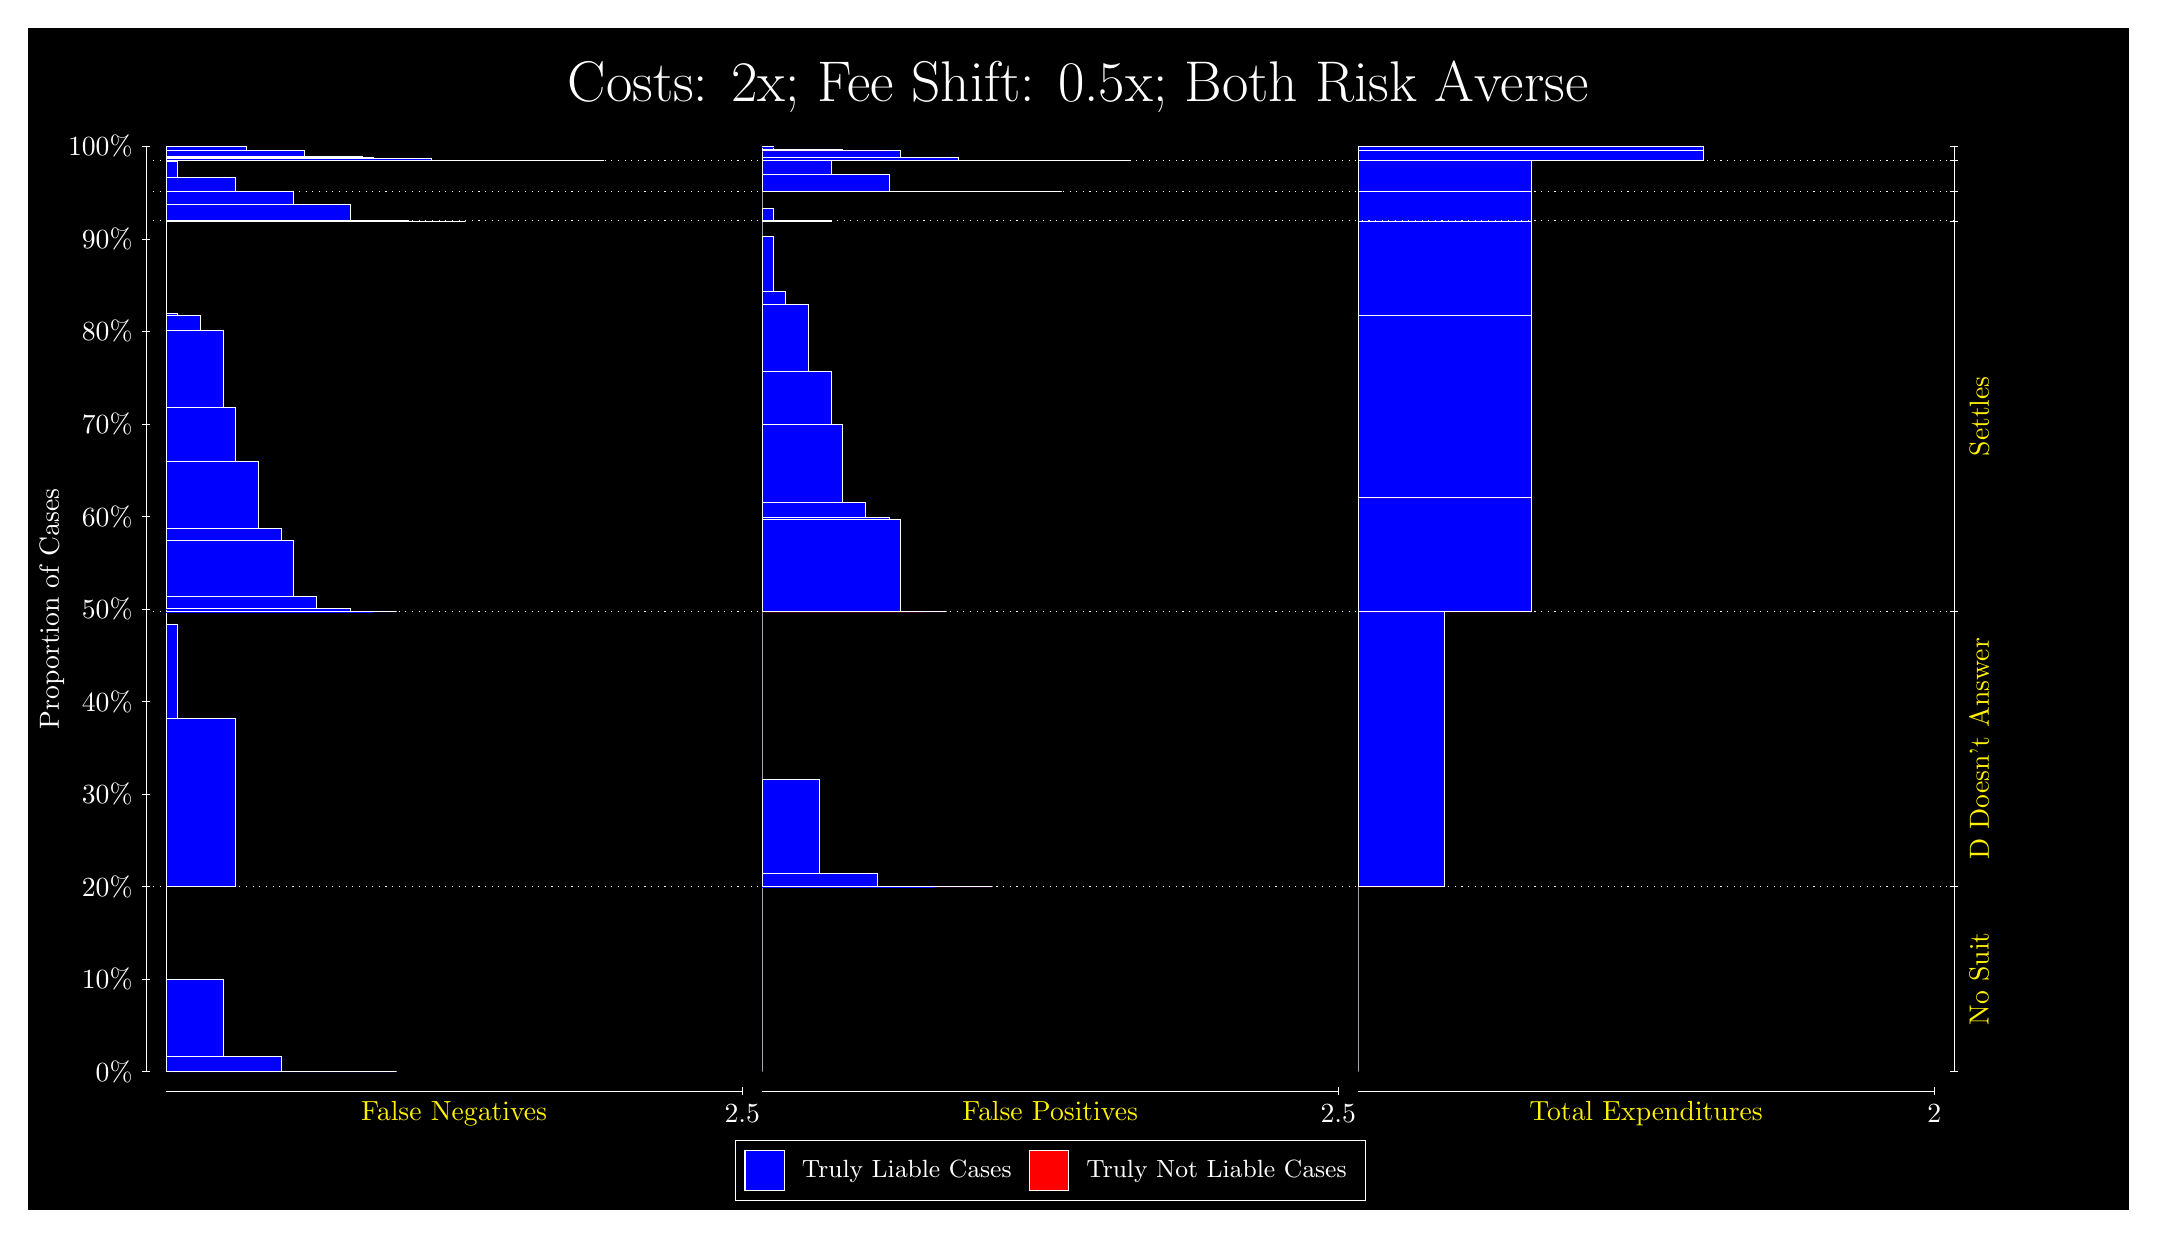
\begin{tikzpicture}
\draw[fill=black] (0,0) rectangle (26.667,15);
\draw[text=white] (0,13.5) rectangle (26.667,15) node[midway] {\huge Costs: 2x; Fee Shift: 0.5x; Both Risk Averse};
\draw[white, very thin] (1.5,1.75) -- (1.5,13.5);
\node[rotate=90, text=white, anchor=center] at (0.3, 7.625) {Proportion of Cases};
\draw[white, very thin] (1.45,1.75) -- (1.55,1.75);
\node[text=white, anchor=east] at (1.45, 1.75) {0\%};
\draw[white, very thin] (1.45,2.925) -- (1.55,2.925);
\node[text=white, anchor=east] at (1.45, 2.925) {10\%};
\draw[white, very thin] (1.45,4.1) -- (1.55,4.1);
\node[text=white, anchor=east] at (1.45, 4.1) {20\%};
\draw[white, very thin] (1.45,5.275) -- (1.55,5.275);
\node[text=white, anchor=east] at (1.45, 5.275) {30\%};
\draw[white, very thin] (1.45,6.45) -- (1.55,6.45);
\node[text=white, anchor=east] at (1.45, 6.45) {40\%};
\draw[white, very thin] (1.45,7.625) -- (1.55,7.625);
\node[text=white, anchor=east] at (1.45, 7.625) {50\%};
\draw[white, very thin] (1.45,8.8) -- (1.55,8.8);
\node[text=white, anchor=east] at (1.45, 8.8) {60\%};
\draw[white, very thin] (1.45,9.975) -- (1.55,9.975);
\node[text=white, anchor=east] at (1.45, 9.975) {70\%};
\draw[white, very thin] (1.45,11.15) -- (1.55,11.15);
\node[text=white, anchor=east] at (1.45, 11.15) {80\%};
\draw[white, very thin] (1.45,12.325) -- (1.55,12.325);
\node[text=white, anchor=east] at (1.45, 12.325) {90\%};
\draw[white, very thin] (1.45,13.5) -- (1.55,13.5);
\node[text=white, anchor=east] at (1.45, 13.5) {100\%};

\draw[white, very thin] (24.457,1.75) -- (24.457,13.5);
\draw[white, very thin] (24.407,1.75) -- (24.507,1.75);
\node[anchor=west] at (24.407, 1.75) {};
\draw[white, very thin] (24.407,4.0995) -- (24.507,4.0995);
\node[anchor=west] at (24.407, 4.0995) {};
\draw[white, very thin] (24.407,7.5919) -- (24.507,7.5919);
\node[anchor=west] at (24.407, 7.5919) {};
\draw[white, very thin] (24.407,12.554) -- (24.507,12.554);
\node[anchor=west] at (24.407, 12.554) {};
\draw[white, very thin] (24.407,12.927) -- (24.507,12.927);
\node[anchor=west] at (24.407, 12.927) {};
\draw[white, very thin] (24.407,13.32) -- (24.507,13.32);
\node[anchor=west] at (24.407, 13.32) {};
\draw[white, very thin] (24.407,13.5) -- (24.507,13.5);
\node[anchor=west] at (24.407, 13.5) {};

\draw[white, very thin, fill=blue] (1.75,1.75) rectangle (4.6775,1.75);
\draw[white, very thin, fill=blue] (1.75,1.75) rectangle (3.9457,1.7516);
\draw[white, very thin, fill=blue] (1.75,1.7516) rectangle (3.2138,1.938);
\draw[white, very thin, fill=blue] (1.75,1.938) rectangle (2.4819,2.9264);
\draw[white, very thin, fill=red] (1.75,2.9264) rectangle (1.75,2.9264);
\draw[white, very thin, fill=blue] (1.75,2.9264) rectangle (1.75,4.0995);
\draw[white, very thin, fill=blue] (1.75,4.0995) rectangle (2.6283,6.2323);
\draw[white, very thin, fill=blue] (1.75,6.2323) rectangle (1.8964,7.4278);
\draw[white, very thin, fill=red] (1.75,7.4278) rectangle (1.75,7.4278);
\draw[white, very thin, fill=blue] (1.75,7.4278) rectangle (1.75,7.5919);
\draw[white, very thin, fill=blue] (1.75,7.5919) rectangle (4.6775,7.5919);
\draw[white, very thin, fill=blue] (1.75,7.5919) rectangle (4.3848,7.5922);
\draw[white, very thin, fill=blue] (1.75,7.5922) rectangle (4.092,7.6281);
\draw[white, very thin, fill=blue] (1.75,7.6281) rectangle (3.9457,7.6286);
\draw[white, very thin, fill=blue] (1.75,7.6286) rectangle (3.6529,7.7832);
\draw[white, very thin, fill=blue] (1.75,7.7832) rectangle (3.3602,8.4918);
\draw[white, very thin, fill=blue] (1.75,8.4918) rectangle (3.2138,8.6531);
\draw[white, very thin, fill=blue] (1.75,8.6531) rectangle (2.921,9.5034);
\draw[white, very thin, fill=blue] (1.75,9.5034) rectangle (2.6283,10.181);
\draw[white, very thin, fill=blue] (1.75,10.181) rectangle (2.4819,11.168);
\draw[white, very thin, fill=blue] (1.75,11.168) rectangle (2.1891,11.355);
\draw[white, very thin, fill=blue] (1.75,11.355) rectangle (1.8964,11.379);
\draw[white, very thin, fill=red] (1.75,11.379) rectangle (1.75,11.379);
\draw[white, very thin, fill=blue] (1.75,11.379) rectangle (1.75,12.554);
\draw[white, very thin, fill=blue] (1.75,12.554) rectangle (5.5558,12.554);
\draw[white, very thin, fill=blue] (1.75,12.554) rectangle (4.8239,12.559);
\draw[white, very thin, fill=blue] (1.75,12.559) rectangle (4.092,12.765);
\draw[white, very thin, fill=blue] (1.75,12.765) rectangle (3.3602,12.925);
\draw[white, very thin, fill=blue] (1.75,12.925) rectangle (2.6283,12.927);
\draw[white, very thin, fill=red] (1.75,12.927) rectangle (1.75,12.927);
\draw[white, very thin, fill=blue] (1.75,12.927) rectangle (2.6283,13.106);
\draw[white, very thin, fill=blue] (1.75,13.106) rectangle (1.8964,13.311);
\draw[white, very thin, fill=red] (1.75,13.311) rectangle (1.75,13.311);
\draw[white, very thin, fill=blue] (1.75,13.311) rectangle (1.75,13.32);
\draw[white, very thin, fill=blue] (1.75,13.32) rectangle (7.3123,13.32);
\draw[white, very thin, fill=blue] (1.75,13.32) rectangle (6.5805,13.32);
\draw[white, very thin, fill=blue] (1.75,13.32) rectangle (5.8486,13.324);
\draw[white, very thin, fill=blue] (1.75,13.324) rectangle (5.7022,13.324);
\draw[white, very thin, fill=blue] (1.75,13.324) rectangle (5.1167,13.352);
\draw[white, very thin, fill=blue] (1.75,13.352) rectangle (4.9703,13.352);
\draw[white, very thin, fill=blue] (1.75,13.352) rectangle (4.3848,13.361);
\draw[white, very thin, fill=blue] (1.75,13.361) rectangle (4.2384,13.375);
\draw[white, very thin, fill=blue] (1.75,13.375) rectangle (3.6529,13.375);
\draw[white, very thin, fill=blue] (1.75,13.375) rectangle (3.5065,13.456);
\draw[white, very thin, fill=blue] (1.75,13.456) rectangle (2.921,13.456);
\draw[white, very thin, fill=blue] (1.75,13.456) rectangle (2.7746,13.498);
\draw[white, very thin, fill=blue] (1.75,13.498) rectangle (2.0428,13.5);
\draw[white, very thin, fill=red] (1.75,13.5) rectangle (1.75,13.5);
\draw[white, very thin, fill=blue] (1.75,13.5) rectangle (1.75,13.5);
\draw[white, very thin, fill=red] (9.3189,1.75) rectangle (9.3189,1.75);
\draw[white, very thin, fill=blue] (9.3189,1.75) rectangle (9.3189,4.0995);
\draw[white, very thin, fill=red] (9.3189,4.0995) rectangle (12.246,4.0995);
\draw[white, very thin, fill=blue] (9.3189,4.0995) rectangle (12.246,4.0995);
\draw[white, very thin, fill=blue] (9.3189,4.0995) rectangle (11.515,4.0998);
\draw[white, very thin, fill=blue] (9.3189,4.0998) rectangle (10.783,4.2636);
\draw[white, very thin, fill=blue] (9.3189,4.2636) rectangle (10.051,5.459);
\draw[white, very thin, fill=blue] (9.3189,5.459) rectangle (9.3189,7.5919);
\draw[white, very thin, fill=red] (9.3189,7.5919) rectangle (11.661,7.5919);
\draw[white, very thin, fill=blue] (9.3189,7.5919) rectangle (11.661,7.5919);
\draw[white, very thin, fill=red] (9.3189,7.5919) rectangle (11.368,7.5919);
\draw[white, very thin, fill=blue] (9.3189,7.5919) rectangle (11.368,7.5938);
\draw[white, very thin, fill=red] (9.3189,7.5938) rectangle (11.075,7.5938);
\draw[white, very thin, fill=blue] (9.3189,7.5938) rectangle (11.075,8.7669);
\draw[white, very thin, fill=blue] (9.3189,8.7669) rectangle (10.929,8.7907);
\draw[white, very thin, fill=blue] (9.3189,8.7907) rectangle (10.636,8.9784);
\draw[white, very thin, fill=blue] (9.3189,8.9784) rectangle (10.344,9.9656);
\draw[white, very thin, fill=blue] (9.3189,9.9656) rectangle (10.197,10.643);
\draw[white, very thin, fill=blue] (9.3189,10.643) rectangle (9.9044,11.493);
\draw[white, very thin, fill=blue] (9.3189,11.493) rectangle (9.6116,11.654);
\draw[white, very thin, fill=blue] (9.3189,11.654) rectangle (9.4652,12.363);
\draw[white, very thin, fill=blue] (9.3189,12.363) rectangle (9.3189,12.554);
\draw[white, very thin, fill=red] (9.3189,12.554) rectangle (10.197,12.554);
\draw[white, very thin, fill=blue] (9.3189,12.554) rectangle (10.197,12.556);
\draw[white, very thin, fill=blue] (9.3189,12.556) rectangle (9.4652,12.716);
\draw[white, very thin, fill=blue] (9.3189,12.716) rectangle (9.3189,12.927);
\draw[white, very thin, fill=red] (9.3189,12.927) rectangle (13.125,12.927);
\draw[white, very thin, fill=blue] (9.3189,12.927) rectangle (13.125,12.927);
\draw[white, very thin, fill=blue] (9.3189,12.927) rectangle (12.393,12.927);
\draw[white, very thin, fill=blue] (9.3189,12.927) rectangle (11.661,12.935);
\draw[white, very thin, fill=blue] (9.3189,12.935) rectangle (10.929,13.141);
\draw[white, very thin, fill=blue] (9.3189,13.141) rectangle (10.197,13.32);
\draw[white, very thin, fill=red] (9.3189,13.32) rectangle (14.003,13.32);
\draw[white, very thin, fill=blue] (9.3189,13.32) rectangle (14.003,13.32);
\draw[white, very thin, fill=red] (9.3189,13.32) rectangle (13.271,13.32);
\draw[white, very thin, fill=blue] (9.3189,13.32) rectangle (13.271,13.32);
\draw[white, very thin, fill=red] (9.3189,13.32) rectangle (12.539,13.32);
\draw[white, very thin, fill=blue] (9.3189,13.32) rectangle (12.539,13.322);
\draw[white, very thin, fill=blue] (9.3189,13.322) rectangle (11.807,13.363);
\draw[white, very thin, fill=red] (9.3189,13.363) rectangle (11.807,13.363);
\draw[white, very thin, fill=blue] (9.3189,13.363) rectangle (11.807,13.363);
\draw[white, very thin, fill=red] (9.3189,13.363) rectangle (11.661,13.363);
\draw[white, very thin, fill=blue] (9.3189,13.363) rectangle (11.661,13.363);
\draw[white, very thin, fill=blue] (9.3189,13.363) rectangle (11.075,13.444);
\draw[white, very thin, fill=blue] (9.3189,13.444) rectangle (11.075,13.444);
\draw[white, very thin, fill=red] (9.3189,13.444) rectangle (10.929,13.444);
\draw[white, very thin, fill=blue] (9.3189,13.444) rectangle (10.929,13.444);
\draw[white, very thin, fill=blue] (9.3189,13.444) rectangle (10.344,13.451);
\draw[white, very thin, fill=blue] (9.3189,13.451) rectangle (10.344,13.458);
\draw[white, very thin, fill=blue] (9.3189,13.458) rectangle (10.197,13.468);
\draw[white, very thin, fill=red] (9.3189,13.468) rectangle (10.197,13.468);
\draw[white, very thin, fill=blue] (9.3189,13.468) rectangle (10.197,13.468);
\draw[white, very thin, fill=blue] (9.3189,13.468) rectangle (9.6116,13.468);
\draw[white, very thin, fill=blue] (9.3189,13.468) rectangle (9.6116,13.468);
\draw[white, very thin, fill=blue] (9.3189,13.468) rectangle (9.4652,13.495);
\draw[white, very thin, fill=blue] (9.3189,13.495) rectangle (9.4652,13.496);
\draw[white, very thin, fill=blue] (9.3189,13.496) rectangle (9.3189,13.5);
\draw[white, very thin, fill=red] (16.888,1.75) rectangle (16.888,1.75);
\draw[white, very thin, fill=blue] (16.888,1.75) rectangle (16.888,4.0995);
\draw[white, very thin, fill=red] (16.888,4.0995) rectangle (17.986,4.0995);
\draw[white, very thin, fill=blue] (16.888,4.0995) rectangle (17.986,7.5919);
\draw[white, very thin, fill=red] (16.888,7.5919) rectangle (19.083,7.5919);
\draw[white, very thin, fill=blue] (16.888,7.5919) rectangle (19.083,9.0373);
\draw[white, very thin, fill=red] (16.888,9.0373) rectangle (19.083,9.0373);
\draw[white, very thin, fill=blue] (16.888,9.0373) rectangle (19.083,11.359);
\draw[white, very thin, fill=red] (16.888,11.359) rectangle (19.083,11.359);
\draw[white, very thin, fill=blue] (16.888,11.359) rectangle (19.083,12.554);
\draw[white, very thin, fill=red] (16.888,12.554) rectangle (19.083,12.554);
\draw[white, very thin, fill=blue] (16.888,12.554) rectangle (19.083,12.927);
\draw[white, very thin, fill=red] (16.888,12.927) rectangle (19.083,12.927);
\draw[white, very thin, fill=blue] (16.888,12.927) rectangle (19.083,13.32);
\draw[white, very thin, fill=red] (16.888,13.32) rectangle (21.279,13.32);
\draw[white, very thin, fill=blue] (16.888,13.32) rectangle (21.279,13.451);
\draw[white, very thin, fill=red] (16.888,13.451) rectangle (21.279,13.451);
\draw[white, very thin, fill=blue] (16.888,13.451) rectangle (21.279,13.5);
\draw[white, dotted] (1.5,4.0995) -- (24.457,4.0995);
\draw[white, dotted] (1.5,7.5919) -- (24.457,7.5919);
\draw[white, dotted] (1.5,12.554) -- (24.457,12.554);
\draw[white, dotted] (1.5,12.927) -- (24.457,12.927);
\draw[white, dotted] (1.5,13.32) -- (24.457,13.32);
\draw[white, very thin] (1.75,1.5) -- (9.0689,1.5);
\node[text=yellow, anchor=north] at (5.4094, 1.5) {False Negatives};
\draw[white, very thin] (9.0689,1.45) -- (9.0689,1.55);
\node[text=white, anchor=north] at (9.0689, 1.45) {2.5};

\draw[white, very thin] (9.3189,1.5) -- (16.638,1.5);
\node[text=yellow, anchor=north] at (12.978, 1.5) {False Positives};
\draw[white, very thin] (16.638,1.45) -- (16.638,1.55);
\node[text=white, anchor=north] at (16.638, 1.45) {2.5};

\draw[white, very thin] (16.888,1.5) -- (24.207,1.5);
\node[text=yellow, anchor=north] at (20.547, 1.5) {Total Expenditures};
\draw[white, very thin] (24.207,1.45) -- (24.207,1.55);
\node[text=white, anchor=north] at (24.207, 1.45) {2};

\node[text=yellow, centered, rotate=90] at (24.777, 2.9247) {No Suit};
\node[text=yellow, centered, rotate=90] at (24.777, 5.8457) {D Doesn't Answer};
\node[text=yellow, centered, rotate=90] at (24.777, 10.073) {Settles};




\draw (12.978300999999998,1.5) node[draw=none] (baseCoordinate) {};
\begin{scope}[align=center]
        \matrix[scale=0.5, draw=white, below=0.5cm of baseCoordinate, nodes={draw}, column sep=0.1cm]{
            \node[rectangle, draw, minimum width=0.5cm, minimum height=0.5cm, fill=blue] {}; &
            \node[draw=none, font=\small, text=white] (B) {Truly Liable Cases}; &
            \node[rectangle, draw, minimum width=0.5cm, minimum height=0.5cm, fill=red] {}; &
            \node[draw=none, font=\small, text=white] (B) {Truly Not Liable Cases}; \\
            };
\end{scope}

\end{tikzpicture}
\end{document}